%% bare_jrnl.tex
%% V1.3
%% 2007/01/11
%% by Michael Shell
%% see http://www.michaelshell.org/
%% for current contact information.
%%
%% This is a skeleton file demonstrating the use of IEEEtran.cls
%% (requires IEEEtran.cls version 1.7 or later) with an IEEE journal paper.
%%
%% Support sites:
%% http://www.michaelshell.org/tex/ieeetran/
%% http://www.ctan.org/tex-archive/macros/latex/contrib/IEEEtran/
%% and
%% http://www.ieee.org/

%%*************************************************************************
%% Legal Notice:
%% This code is offered as-is without any warranty either expressed or
%% implied; without even the implied warranty of MERCHANTABILITY or
%% FITNESS FOR A PARTICULAR PURPOSE! 
%% User assumes all risk.
%% In no event shall IEEE or any contributor to this code be liable for
%% any damages or losses, including, but not limited to, incidental,
%% consequential, or any other damages, resulting from the use or misuse
%% of any information contained here.
%%
%% All comments are the opinions of their respective authors and are not
%% necessarily endorsed by the IEEE.
%%
%% This work is distributed under the LaTeX Project Public License (LPPL)
%% ( http://www.latex-project.org/ ) version 1.3, and may be freely used,
%% distributed and modified. A copy of the LPPL, version 1.3, is included
%% in the base LaTeX documentation of all distributions of LaTeX released
%% 2003/12/01 or later.
%% Retain all contribution notices and credits.
%% ** Modified files should be clearly indicated as such, including  **
%% ** renaming them and changing author support contact information. **
%%
%% File list of work: IEEEtran.cls, IEEEtran_HOWTO.pdf, bare_adv.tex,
%%                    bare_conf.tex, bare_jrnl.tex, bare_jrnl_compsoc.tex
%%*************************************************************************

\documentclass[journal]{IEEEtran}

\newcommand{\subparagraph}{}

\usepackage{amsmath,
            amssymb,
            amsthm,
            atbegshi,
            caption,
            subcaption,
            epigraph,
            etoolbox,
            enumitem,
            fancyhdr,
            geometry,
            graphicx,
            hyperref,
            kpfonts,
            lipsum,
            longtable,
            natbib,
            tabulary,
            thmtools,
            tikz,
            tikzpagenodes,
            titletoc,
            titlesec,
            tocloft,
            url,
            wrapfig
}
\usepackage[utf8]{inputenc}


\begin{document}
%
% paper title
% can use linebreaks \\ within to get better formatting as desired
\title{Solving Puzzles with A*-GAC}

\author{Anders Sildnes, Andrej Leitner~\IEEEmembership{students }% <-this % stops a space. jobtitle in memberkj
}% \thanks{Utsendt 2014}}

% The paper headers
\markboth{Solving Puzzles with A*-GAC}%
{h}

% make the title area
\maketitle

\begin{abstract}
    This text answers assignment 3, 4: Combining Best-First Search and Constraint-Satisfaction to Solve Complex Puzzles.  
    In this document, we explain representations, heuristics and design decisions we used to handle flow puzzels and nonograms tasks. 
    The assignment is built on previous module using simple extensions and subclassing.
\end{abstract}

% \begin{IEEEkeywords}
%     Stuff
% \end{IEEEkeywords}
\IEEEPARstart{C}{SP} solutions defines variables with domains.
A valid solution is one where the domain of all variables has been reduced to the
singleton domain. This occurs by making sure that a) no constraints are violated
and b) all variables are iterated over, and been locked to a single value in their
domain.

\section*{Generality of A*-GAC Solver}
The solvers for each puzzle is implemented using the same source code as in
the previous project. \textit{Essentially}, we use the exact same code for out 
CNET\footnote{ConstraintNETwork, explained in project 1}. The changes we have made
are:
\begin{enumerate}
    \item Added methods ``addCons(...)'' and ``addLambda(...)'', which can take
        either a lambda, or a string that is parsable as a lambda, and translate
        that into a constraint. 
        Example: addCons([1,2], "A \textless B") adds a constraint between VI
        1 and 2, where the indexes are mapped into the string
        in order (the first index maps
        to the first capital letter in the string).
    \item Special case handling for when the domains consist of \textit{sets} rather
        than single numbers, as used in the previous assignment.
\end{enumerate}
Apart from item 1 and 2, this assignement is solved by subclassing the class
``Problem'' and implementing its abstract methods\footnote{in ``astar.py'': triggerStart(), genNeighbour(), destructor(), updateStates()}
. Also, you will need to parse the input for each problem. This is done in our
``main.py''. As a reminder, the abstract methods of the ``Problem'' class
defines:
\begin{description}
    \item[Drawing] - how each state should be painted. The method receives 
        both the previous state and the current one. By comparing the states, you
        can avoid repainting the whole GUI, or use a lazy updating scheme.
        In this assignement, with either few states or nodes, we chose the latter.
    \item[Destructor] - what to do when the A* queue is exhausted. In this assigment
        we simply print the total number of nodes used and expanded in the
        A*-search, and do a last repainting of the GUI.
    \item[Generating successor states] - defines how, given a state, to generate
        all its successors.
    \item[Generating initial state] - creates the initial queue for A*.
\end{description}


\subsection*{Considerations}
The biggest problem we found related to using A*-GAC was that we could not
implement a solution that relied on states.
For example, apart from running time, it should not matter if a constraint
$c_1$  is run before constraint $c_2$ - they should both prune their domain as
much as needed. Therefore we could not implement thoughts such as
``if check(A) then othercheck (B)''.

Both problems could be fully expressed as SAT, so we found both problems to
be NP-hard. Therefore we knew that to find exact solutions, we would have
non-polyomial problem-sizes. It was therefore tempting to use local search,
but we felt that the inputs given were small enough that an iterative solution
would do well.

\section*{Modelling Nonograms}
While nonograms certainly can be expressed as SAT, we found it easier to
follow the model suggested to us in the assignment text. This is 
to use each row or column as a VI, and have their domains as all possible
orderings given their rule $r$. The disadvantage of this approach, namely the large domain-spaces, were not deemed
to be critical to our application under the premise that we would always solve
relatively small boards.

Each cell in the cartesian-grid used in a nonogram can be represented by a single number.
We did this numbering in the fashion seen in ~\autoref{fig:grid}.
% We used cell numbering such that a cell at row i, column j has coordinate 
% $(\text{WIDTH} \times i) + j$.
% Therefore, a board with $3 \times 3$ cells will have numbers 1-9 for each position.
Now the possible domain for each row, column is represented by the numbers
in that row or column. For example, given the rule ``3'', the rows in  ~\autoref{fig:grid} would
have their domain as [1,2,3] or [4,5,6].
Blank cells are representing by using the negative of the coordinate in a cell.
Thus, for the second column in ~\autoref{fig:grid}, given rule ``1'', would have
two possible domain values: [-2,4] and [2,-4].

\begin{figure}[Hb]
\centering
  % TikZ picture with origin upper left
    \begin{tikzpicture}[yscale=-1] 
        % 4x4 grid
        \draw (0, 0) grid (3, 2);
        % origin point
        \draw [color=blue, fill=blue] (0, 0) circle (0.1);
        % % x-axis
        % \draw [thick,->] (0, 0) -- (3.5, 0);
        % % y-axis
        % \draw [thick,->] (0, 0) -- (0, 3.5);
        % origin label
        % \node at (-0.5, 0.5) {1};
        \node at (0.5, 0.5) {1};
        \node at (1.5, 0.5) {2};
        \node at (2.5, 0.5) {3};
        \node at (0.5, 1.5) {3};
        \node at (1.5, 1.5) {4};
        \node at (2.5, 1.5) {5};
        % % x-axis label
        % \node at (4.5, -0.5) {200px};
        % % y-axis label
        % \node at (0, 5) {200px};
    \end{tikzpicture}
    \caption{Our representation of a cartesian grid}
\label{fig:grid}
\end{figure}

Now, all constraints can be expressed as matchings between two VI's,
a row and a column. In pseudocode, our generated lambda is as follows:
\begin{verbatim}
len(A.intersection(B)) == 1
\end{verbatim}

where A,B can be the VI for a row or column (the function is symmetric).

An intersection will only occur if the shared coordinate in each domain has the same
sign (positive or negative value). Since each row and column only share one cell,
this function is able to filter domains successfully.

The disadvantage to our lambda is that the constraints will assess large spaces,
while the constraint only depend on one value in each domain. Also,
the A*-GAC requires much copying states and domains, so much excess overhead
is included. However, the program still runs in under 20 seconds for all 
the given test inputs, so we have not spent time optimizing the function\footnote{
    using properties such as that you can determine exactly which cell you need
to compare using only the indexes $i,j$}.

% Firstly we pair each row with all columns 
% and then we pass through these pairs with intersection checking. In particular, we check for the length of intersection 
% between possible row and column pattern and accept only value $1$ as valid solution. % DO WE? eval_value is not used anywhere, only intersection?
%
\subsection{Choice of heuristic}
After finishing our solver, it was easy to see that few states are ever created and
expanded. This is due to the coupling of constraints: each row is paired
with every column, and vice versa. In general this means that reducing one domain forces
the GAC to filter the entire space of VI's multiple times.
With a small problem space for the A*-algorithm, it became clear that the
choise of heuristic is not critical. We used ``min-domain'', which works OK.

% In this approach we can find heuristics in some places:
% \begin{enumerate}
%     \item in A* we used the same $h-function$ as in previous graph coloring module where an index value to each node 
%     in the search tree is given determined by:
%     \begin{verbatim}
%      f = depth + h(domains)
%      \end{verbatim}
%      In $h-function$ we count the size of all domains to each variable and then the state with lowest value is chosen.\\
\subsection{Choice of next VI}
We tried experimenting with the choice of each VI. We initially postulated that
choosing a center row or column would yield would be faster. However, it is
important to note that to the constraints only binary relationships matter,
and pruning one row will likely invoke constraints from all other rows.
Therefore the starting VI is chosen randomly.

For successor states we found that selecting the VI with the smallest domain
reduced the running time. The idea is that this VI first of all has fewer
constraints that needs to be checked. Also, assuming our heuristic has chosen
a state that is closer to the goal, the VI with the smallest domain will likely
force a feasible solution faster.

\section*{Modeling Flow Puzzles}
We chose to use SAT representation for the flow puzzle. 
While the benchmark of Michael Spivey 
\small\begin{verbatim}
[http://spivey.oriel.ox.ac.uk
/corner/Programming_competition_results]\end{verbatim}
\normalsize
found that it can be faster to represent point in the graph by its
incoming/outgoing direction of flow (NE, NW, NS, WE, WS \dots), 
we chose SAT because of its simplicity and ease of implementing it in our
model, and also with the knowledge that the input files were no bigger than
$10 \times 10$, and that small differences in performance is not critical to our evaluation.
Also, the SAT formulation meant that we had small domains, which is important
when using our CNET because domains are copied quite often... So therefore, 
even if the winning ``numberlink'' from the benchmark[ibid] modeled 
his project using directions, it might be that it is inefficient in 
our model when using GAC and constraint propagation.

In our model, we represent the board as a 2D-grid of cells, each representing one
vertex instance $v_{i,j}$ for position $i,j$ in the cartesian plane.
For each $v$, you can assign $k$ colors, where $k$ is given by
the number of endpoints / 2. 
Each cell $v_{i,j}$ must be a part of the path
\footnote{I will assume the reader is has a mutual understanding of ``path''}
from an endpoint $e_{i,j}$ to another endpoint $e_{i+\alpha,j+\beta}$.
Therefore our constraints are modelled as follows:
\begin{align}
    \forall{i,j}: leastTwoOf( v_{i+1,j},v_{i+1,j},v_{i+1,j},v_{i+1,j}, ) == v_{i,j} \\   %ALL arguments are same
    \forall{i,j}: leastOneOf( v_{i+1,j},v_{i+1,j},v_{i+1,j},v_{i+1,j}, ) == e_{i,j}
\end{align}
this can also be thought of as applying a 5-point stencil to the grid
and validating each neighbour value. This constraint only applies to the entir
LOOPS, deffered

\begin{figure}[Hb]
\centering
    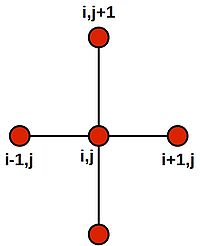
\includegraphics[height=2cm,keepaspectratio,width=2.5in]{stencil.jpg}
\caption{Stencil operation}
\label{fig:stencil}
\end{figure}

\subsection{Choice of next cell}
Clearly, random is bad..

\subsection{Choice of heurstic}
We scanned through 

\begin{figure}[Hb]
\centering
    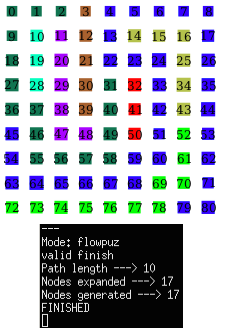
\includegraphics[keepaspectratio, height=8cm]{flowpuz.png}
\caption{Flowpuzzle example}
\label{fig:Flowpuzzle}
\end{figure}

\begin{figure}[Hb]
\centering
    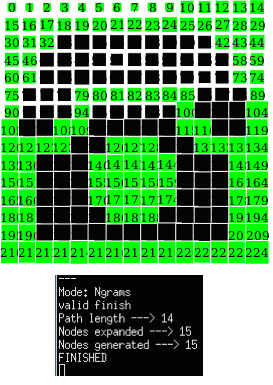
\includegraphics[keepaspectratio, height=8cm]{ngram.png}
\caption{Nonogram example}
\label{fig:Nonogram}
\end{figure}




\end{document}
% Same for columns. We do this with recursive function $generatePos$ inspired by
% this project: \small\begin{verbatim}
% [https://github.com/coolbutuseless
% /nonogram-solver]
% \end{verbatim}
% \normalsize

% Here we are able to build the CNET. In this step we had to create a new subclass of CNET with 
% overridden constructor. Just because we use variables with constant domain size in previous modules 
% and this case we work with variable domain size.
